\documentclass[t]{beamer}

\subtitle{Section 2.3: Subgroups}

\usepackage{amsthm,amsmath,amsfonts,hyperref,graphicx,color,multicol,soul}
\usepackage{enumitem,tikz,tikz-cd,setspace,mathtools}

%%%%%%%%%%
%Beamer Template Customization
%%%%%%%%%%
\setbeamertemplate{navigation symbols}{}
\setbeamertemplate{theorems}[ams style]
\setbeamertemplate{blocks}[rounded]

\definecolor{Blu}{RGB}{43,62,133} % UWEC Blue
\setbeamercolor{structure}{fg=Blu} % Titles

%Unnumbered footnotes:
\newcommand{\blfootnote}[1]{%
	\begingroup
	\renewcommand\thefootnote{}\footnote{#1}%
	\addtocounter{footnote}{-1}%
	\endgroup
}

%%%%%%%%%%
%TikZ Stuff
%%%%%%%%%%
\usetikzlibrary{arrows}
\usetikzlibrary{shapes.geometric}
\tikzset{
	smaller/.style={
		draw,
		regular polygon,
		regular polygon sides=3,
		fill=white,
		node distance=2cm,
		minimum height=1in,
		line width = 2pt
	}
}
\tikzset{
	smsquare/.style={
		draw,
		regular polygon,
		regular polygon sides=4,
		fill=white,
		node distance=2cm,
		minimum height=1in,
		line width = 2pt
	}
}


%%%%%%%%%%
%Custom Commands
%%%%%%%%%%

\newcommand{\C}{\mathbb{C}}
\newcommand{\quats}{\mathbb{H}}
\newcommand{\N}{\mathbb{N}}
\newcommand{\Q}{\mathbb{Q}}
\newcommand{\R}{\mathbb{R}}
\newcommand{\Z}{\mathbb{Z}}

\newcommand{\ds}{\displaystyle}

\newcommand{\fn}{\insertframenumber}

\newcommand{\id}{\operatorname{id}}
\newcommand{\im}{\operatorname{im}}
\newcommand{\Aut}{\operatorname{Aut}}
\newcommand{\Inn}{\operatorname{Inn}}

\newcommand{\blank}[1]{\underline{\hspace*{#1}}}

\newcommand{\abar}{\overline{a}}
\newcommand{\bbar}{\overline{b}}
\newcommand{\cbar}{\overline{c}}

\newcommand{\nml}{\unlhd}

%%%%%%%%%%
%Custom Theorem Environments
%%%%%%%%%%
\theoremstyle{definition}
\newtheorem{exercise}{Exercise}
\newtheorem{question}[exercise]{Question}
\newtheorem{warmup}{Warm-Up}
\newtheorem*{defn}{Definition}
\newtheorem*{exa}{Example}
\newtheorem*{disc}{Group Discussion}
\newtheorem*{nb}{Note}
\newtheorem*{recall}{Recall}
\renewcommand{\emph}[1]{{\color{blue}\texttt{#1}}}

\definecolor{Gold}{RGB}{237, 172, 26}
%Statement block
\newenvironment{statementblock}[1]{%
	\setbeamercolor{block body}{bg=Gold!20}
	\setbeamercolor{block title}{bg=Gold}
	\begin{block}{\textbf{#1.}}}{\end{block}}
\newenvironment{thm}[1]{%
	\setbeamercolor{block body}{bg=Gold!20}
	\setbeamercolor{block title}{bg=Gold}
	\begin{block}{\textbf{Theorem #1.}}}{\end{block}}


%%%%%%%%%%
%Custom Environment Wrappers
%%%%%%%%%%
\newcommand{\enumarabic}[1]{
	\begin{enumerate}[label=\textbf{\arabic*.}]
		#1
	\end{enumerate}
}
\newcommand{\enumalph}[1]{
	\begin{enumerate}[label=(\alph*)]
		#1
	\end{enumerate}
}
\newcommand{\bulletize}[1]{
	\begin{itemize}[label=$\bullet$]
		#1
	\end{itemize}
}
\newcommand{\circtize}[1]{
	\begin{itemize}[label=$\circ$]
		#1
	\end{itemize}
}
\newcommand{\slide}[1]{
	\begin{frame}{\fn}
		#1
	\end{frame}
}
\newcommand{\slidec}[1]{
\begin{frame}[c]{\fn}
	#1
\end{frame}
}
\newcommand{\slidet}[2]{
	\begin{frame}{\fn\ - #1}
		#2
	\end{frame}
}


\newcommand{\startdoc}{
		\title{Math 425: Abstract Algebra 1}
		\author{Mckenzie West}
		\date{Last Updated: \today}
		\begin{frame}
			\maketitle
		\end{frame}
}

\newcommand{\topics}[2]{
	\begin{frame}{\insertframenumber}
		\begin{block}{\textbf{Last Section.}}
			\begin{itemize}[label=--]
				#1
			\end{itemize}
		\end{block}
		\begin{block}{\textbf{This Section.}}
			\begin{itemize}[label=--]
				#2
			\end{itemize}
		\end{block}
	\end{frame}
}

\begin{document} 
	\startdoc
	
	\topics{ 
		\item Groups
		\item Properties of Groups
	}
	{
		\item Subgroups
		\item The Subgroup Test
		\item The center of a group, $Z(G)$
	}
\slide{
	\begin{defn}
		A subsets $H$ of a group $G$ is call a \emph{subgroup} of $G$ if $H$ is also a group using the same operation as $G$.
		We denote subgroups using the notation $H\leq G$.
		
		If $H\leq G$ and $H\neq G$, we call $H$ a \emph{proper subgroup of G}.
	\end{defn}
	\begin{exa}
		Every group $G$ with two or more elements automatically has two subgroups:
			\enumalph{\item $G\leq G$\item $\{e\}\leq G$ (the \emph{trivial subgroup})}
	\end{exa}
}

\slide{
	\begin{exa}
		\enumalph{
			\setlength{\itemsep}{.5in}
			\item $(\Z,+)$ is a subgroup of $(\R,+)$
			\item $\Z\leq\Q\leq\R\leq\C$
			\item $(A_3,\circ)$ is a subgroup of $(S_3,\circ)$
			
				Recall: $S_3=\{\varepsilon,(1\ 2),(1\ 3),(2\ 3),(1\ 2\ 3),(1\ 3\ 2)\}$ and
				$A_3=\{\varepsilon,(1\ 2\ 3),(1\ 3\ 2)\}$
		}
	\end{exa}
}

\slide{
	\begin{picture}(0,0)
	\put(150,-50){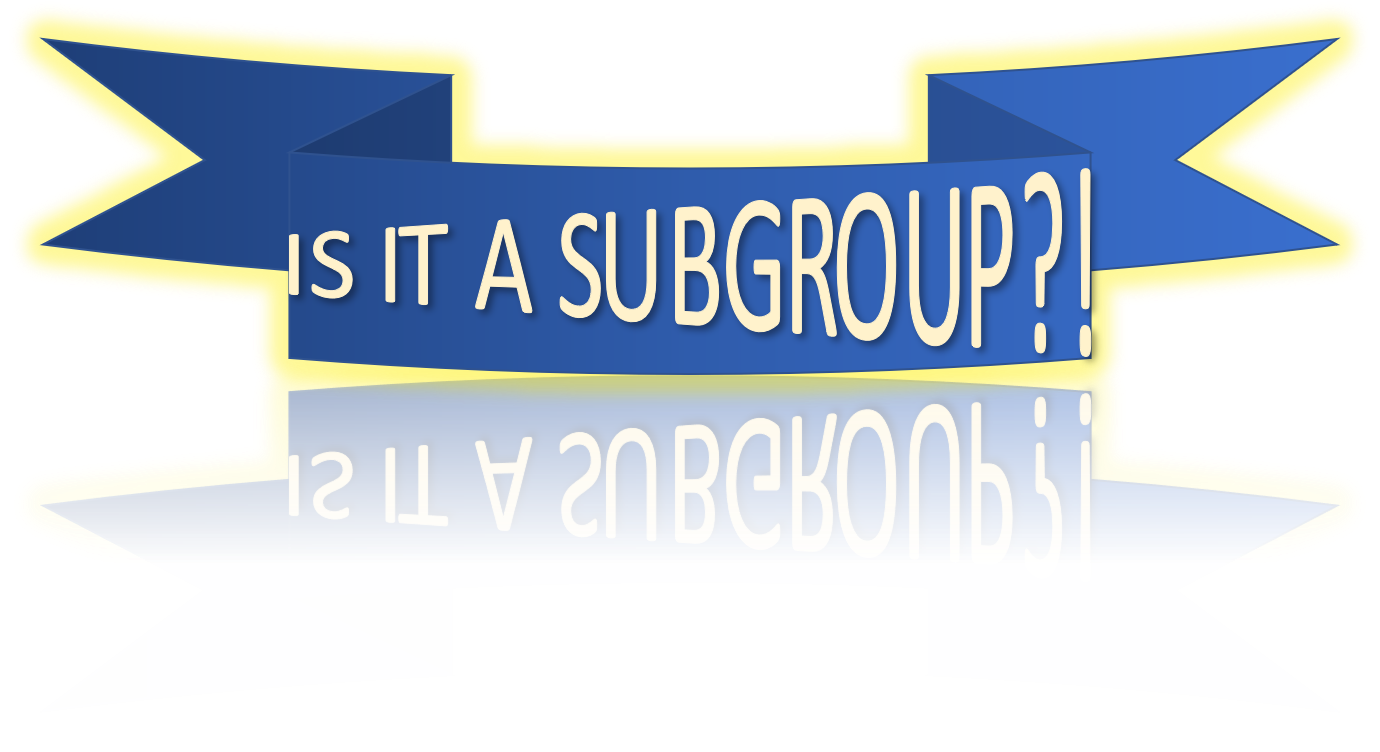
\includegraphics[width=2in]{subgroup_game}}
	\end{picture}
	\begin{exercise}
		Is it a Subgroup?!
		
		\[\text{Is }(\Q\setminus\{0\},\cdot)\leq (\R,+)?\]
		\vskip 1in\mbox{}
	\end{exercise}
}
\slide{
	\begin{picture}(0,0)
	\put(150,-50){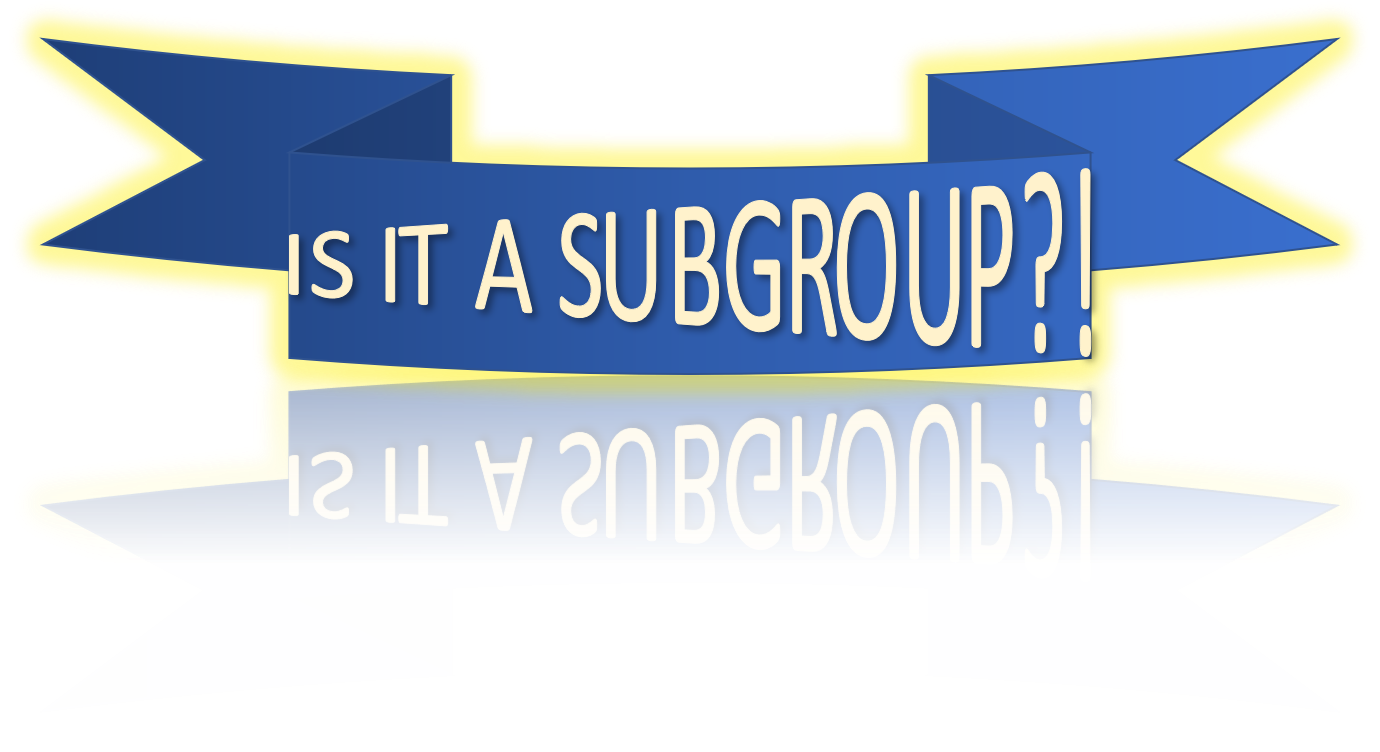
\includegraphics[width=2in]{subgroup_game}}
	\end{picture}
	\begin{exercise}
		Is it a Subgroup?!
		
		\[\text{Is }(\{\bar0,\bar2\},+)\leq (\Z_4,+)?\]
		\vskip 1in\mbox{}
	\end{exercise}
}
\slide{
\begin{picture}(0,0)
\put(150,-50){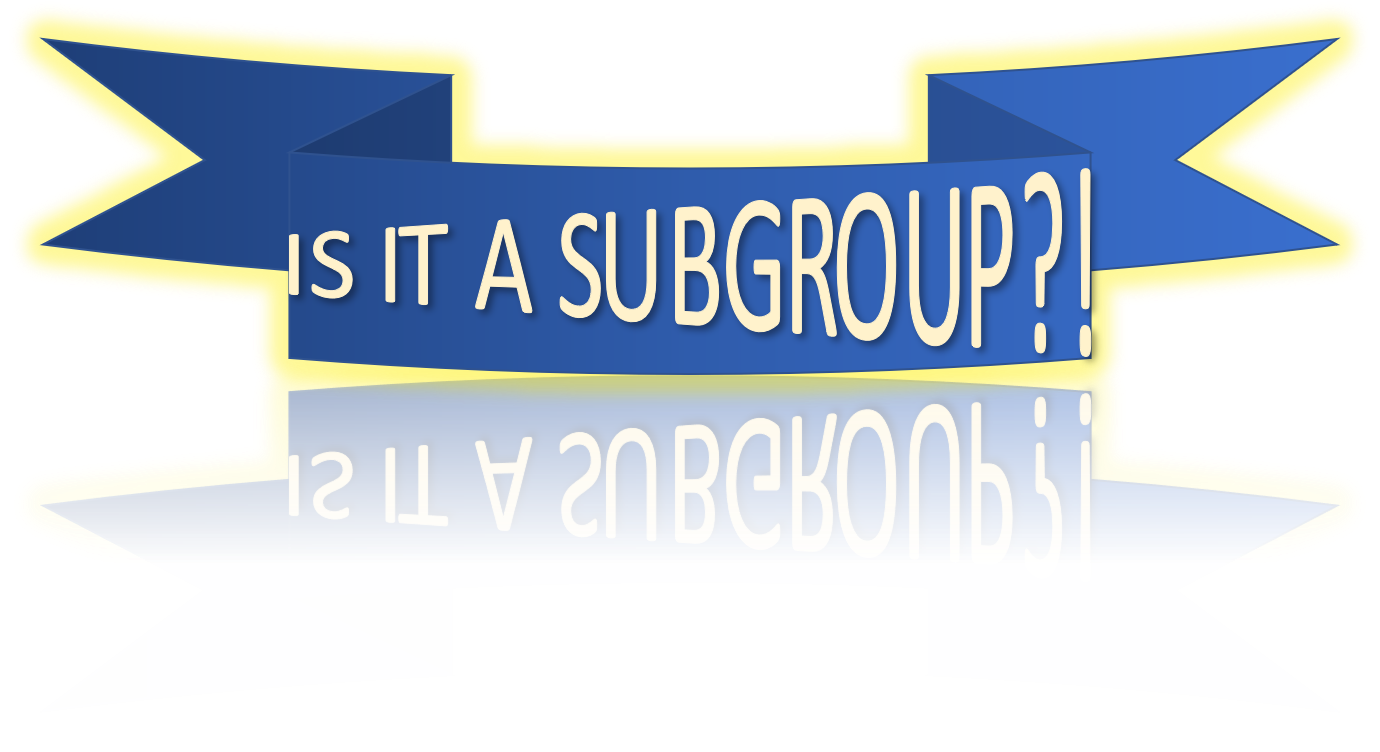
\includegraphics[width=2in]{subgroup_game}}
\end{picture}
\begin{exercise}
	Is it a Subgroup?!
	
	\[\text{Is }(\Z_2,+)\leq (\Z_3,+)?\]
	\vskip 1in\mbox{}
\end{exercise}
}
\slide{
	\begin{picture}(0,0)
	\put(150,-50){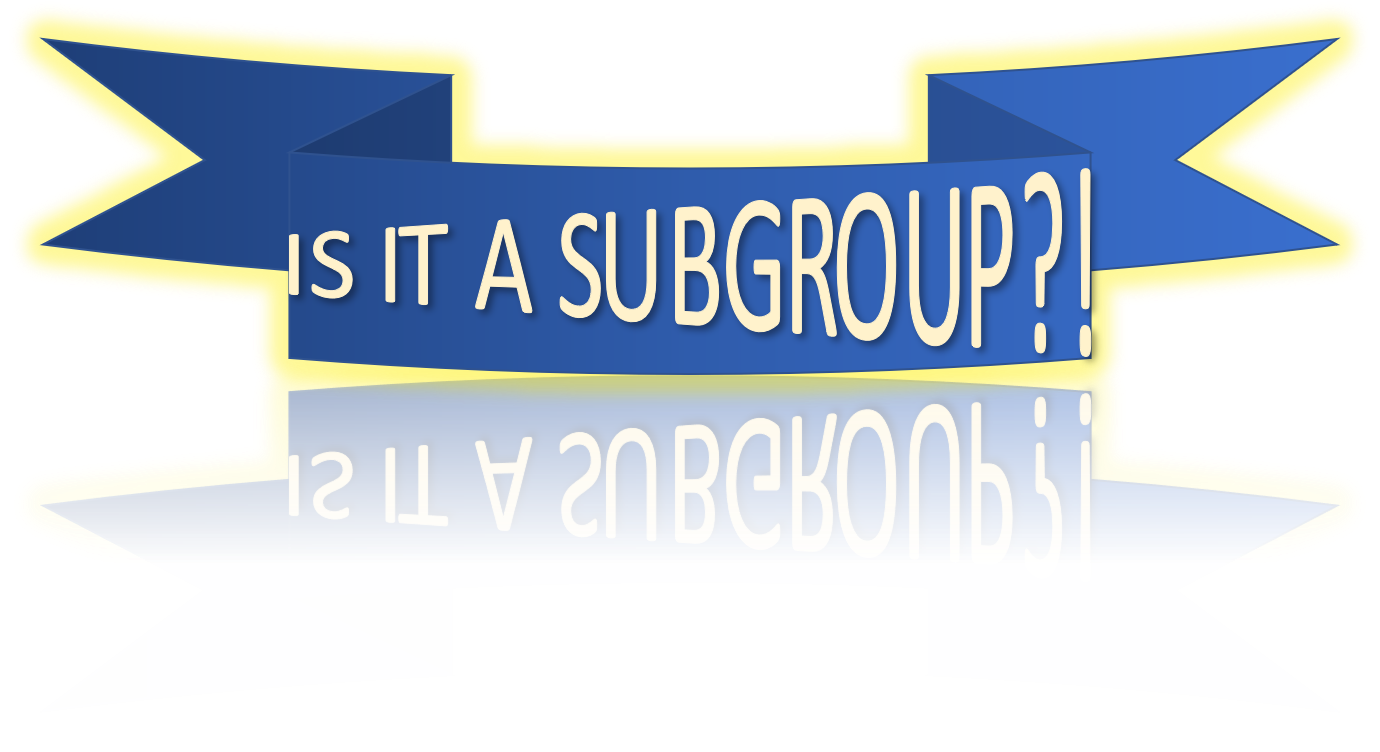
\includegraphics[width=2in]{subgroup_game}}
	\end{picture}
\begin{exercise}
	Is it a Subgroup?!
	
	\[\text{Is }(\{i,-i\},\cdot)\leq (\mathcal{U}_4,\cdot)?\]
	
	Recall $\mathcal{U}_4=\{1,i,-1,-i\}$.
		\vskip 1in\mbox{}
\end{exercise}
}
\slide{
	\begin{picture}(0,0)
	\put(150,-50){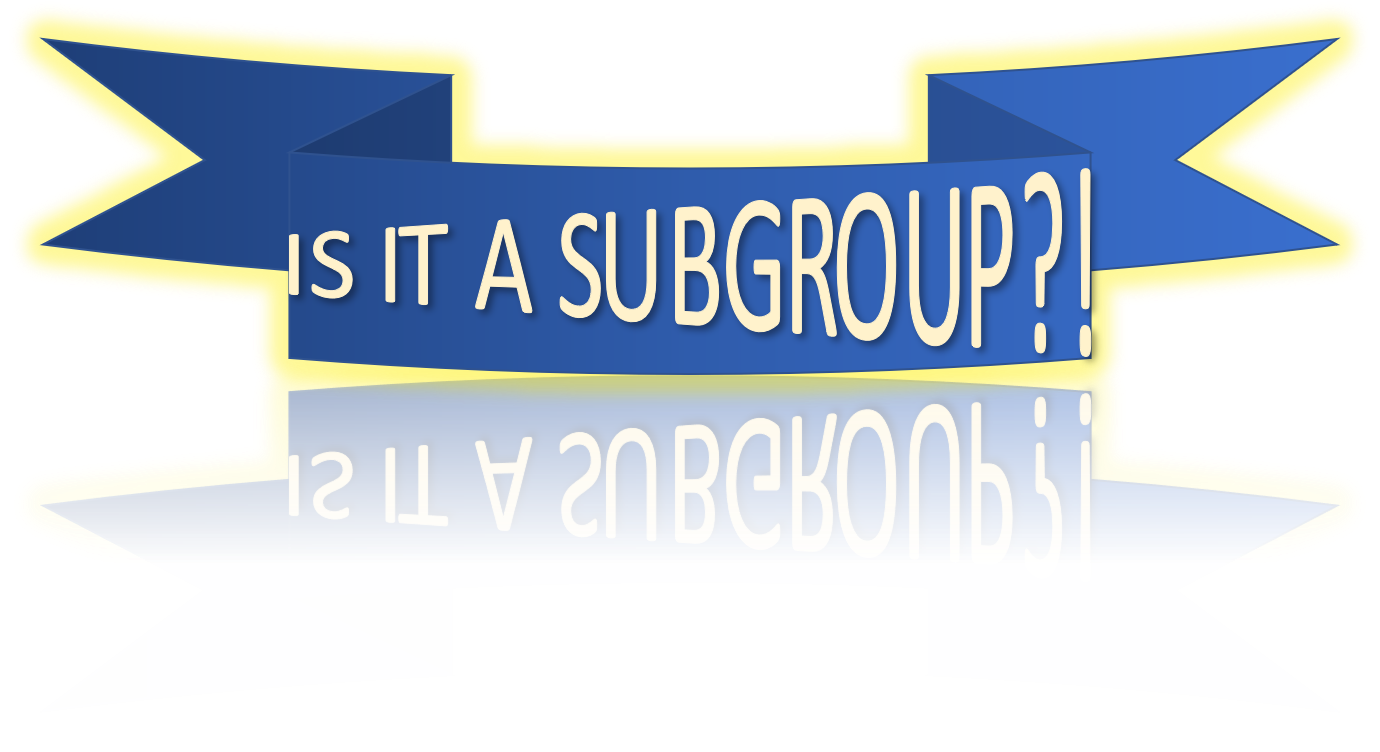
\includegraphics[width=2in]{subgroup_game}}
	\end{picture}
\begin{exercise}
	Is it a Subgroup?!
	\[\text{Is }(\Z_2,+)\leq (\Z_2\times\Z_2,\text{component-wise }+)?\]
	\vskip 1in\mbox{}
\end{exercise}
}
\slide{
\begin{picture}(0,0)
\put(150,-50){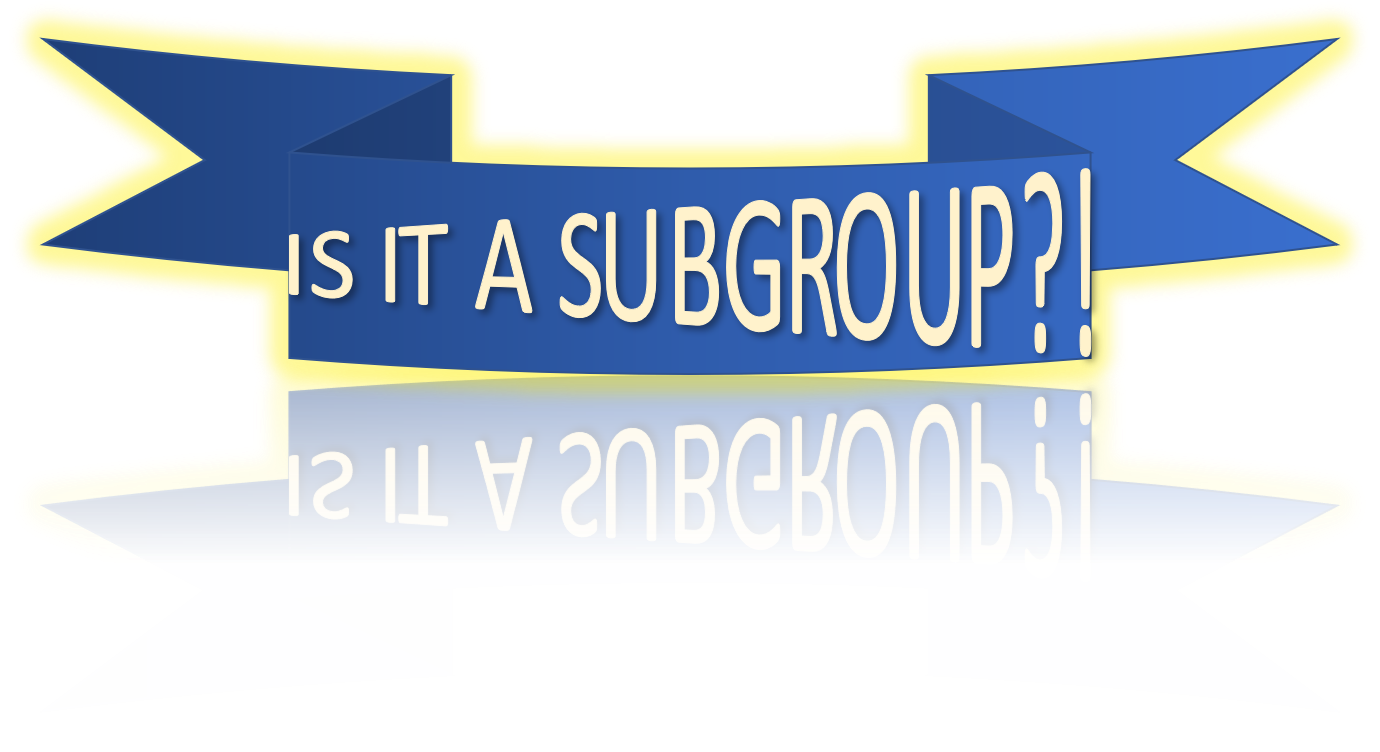
\includegraphics[width=2in]{subgroup_game}}
\end{picture}
\begin{exercise}
	Is it a Subgroup?!
	\[\text{Is }(\{\varepsilon,(1\ 2)\},\circ)\leq (S_3,\circ)?\]
	\vskip 1in\mbox{}
\end{exercise}
}
%\slide{
%	\begin{minipage}{1.5in}
%		\begin{block}{\textbf{Brain Break.}}
%		\enumarabic{\item Starburst\item Skittles \item Dots \item Airheads\item Laffy Taffy}
%	\end{block}
%	\end{minipage}
%	\begin{minipage}{2in}
%		\includegraphics[width=2in]{images/fruity_candy}
%	\end{minipage}
%}
\slide{
\begin{statementblock}{Subgoup Test (Theorem 2.3.1)}
	A subset $H$ of a group $G$ is a subgroup of $G$ if and only if the following conditions are satisfied.
	\enumarabic{
		\item $1_G\in H$, where $1_G$ is the identity element of $G$.
		\item If $h\in H$ and $h_1\in H$, then $hh_1\in H$.
		\item If $h\in H$, then $h^{-1}\in H$, where $h^{-1}\in G$ denotes the inverse of $h$ in $G$.
	}
	
	Note that implicit in these statements, if $H\leq G$ then $H$ and $G$ have the same unity and inverses persist.
\end{statementblock}
}
\slide{
	\begin{exercise}
		Show $(2\Z,+)\leq(\Z,+)$ using the subgroup test.
		\vskip 2in\mbox{}
	\end{exercise}
}
\slide{
	\begin{exercise}
		Is $(2\Z+1,+)\leq (\Z,+)$?
		\vskip 2in\mbox{}
	\end{exercise}
}
\slide{
	\begin{exercise}
		We have the \emph{special linear group} and \emph{general linear group}, respectively below:
			\[SL_2(\R)=\{M\in Mat_n(\R) | \det M=1\},\]
			\[GL_2(\R)=\{M\in Mat_n(\R) | \det M\neq 0\}.\]
		Show $(SL_2(\R),\cdot)\leq (GL_2(\R),\cdot)$
	\end{exercise}
	\vskip 1.5in\mbox{}
}


%\slide{
%\begin{defn}
%	The \emph{subset of $G$ generated by $g\in G$} in multiplicative notation is
%	\[\langle g\rangle=\{g^k | k\in Z\}=\{\dots,g^{-1}*g^{-1},g^{-1},e,g,g*g,g*g*g\dots\}.\]
%	The \emph{subset of $G$ generated by $g\in G$} in additive notation is
%	\begin{align*}
%		\langle g\rangle&=\{kg | k\in Z\}.
%	\end{align*}
%\end{defn}
%}
%\slide{
%\begin{exercise}
%	What does is the subset $\langle 2\rangle$ of $\Z$ look like?
%	\vskip .75in
%	What does is the subset $\langle 3\rangle$ of $\Z$ look like?
%	\vskip .75in
%	What does is the subset $\langle n\rangle$ of $\Z$ look like?
%\end{exercise}
%}
%\slide{
%\begin{statementblock}
%	Prove that if $G$ is a group and $g\in G$, then $\langle g\rangle$ is a subgroup of $G$.
%\end{statementblock}
%}
%\slide{
%\begin{exercise}
%	Let $G=(\Z_6,+)$, then $\langle\overline{4}\rangle \leq G$.  Describe $\langle\overline{4}\rangle$.\vskip .75in\mbox{}
%\end{exercise}
%\begin{exercise}
%	Let $G=(\Z_2\times\Z_2,+)$, then $\langle(\overline{0},\overline{1})\rangle \leq G$.  Describe $\langle({0},\overline{1})\rangle$.\vskip .75in\mbox{}
%\end{exercise}
%}
%\slide{
%\begin{defn}
%	The \emph{subgroup lattice} of a group $G$ is a schematic picture of the subgroups of $G$.  A line going up from one group to another indicates that the bottom group is a subgroup of the top one.
%\end{defn}
%\begin{exa}
%	Subgroup Lattices for $\{e\}, \Z_2$, and $\Z_3$.\vskip 1em
%\end{exa}
%}
%\slide{
%\begin{nb}
%	Recall that there were two groups of order 4, $\Z_4$ and $\Z_2\times \Z_2$.  We call $\Z_4$ the \emph{cyclic group of order 4} and we call $\Z_2\times \Z_2$ the \emph{Klein-4 Group}, denoted $K_4$.
%\end{nb}
%\begin{exercise}
%	Determine all of the subgroups of $\Z_4$ and of $K_4$ and draw a subgroup lattice for each.\vskip 1.5in\mbox{}
%\end{exercise}
%}
%\slide{
%\begin{exercise}
%	What are the subgroups of \[S_3=\{e,(1\ 2),(1\ 3), (2\ 3),(1\ 2\ 3),(1\ 3\ 2)\}?\]  Draw a subgroup lattice.
%\end{exercise}
%}
\slide{
\begin{defn}
	The \emph{center} of the group $G$ is the set
	\[Z(G) = \{z\in G|zg=gz\ \forall g\in G\}.\]
\end{defn}
\begin{question}
	How would you describe $Z(G)$ with words?
\end{question}
}
\slide{
\begin{thm}{2.3.3}
	If $G$ is any group, then $Z(G)$ is a subgroup of $G$. 
	
	Moreover, $Z(G)$ is always abelian.
\end{thm}
\begin{proof}\renewcommand{\qedsymbol}{}
	\begin{itemize}[label=$\bullet$]
		\setlength{\itemsep}{.5in}
		\item (Identity) 
		\item (Closure) 
		\item (Inverses)
		\item[$\circ$] (Abelian)
	\end{itemize}
\end{proof}
}
\slide{
	\begin{defn}
		Given $H\leq G$ and $g\in G$, we define the set
		\[{\color{blue} gHg^{-1}} = \{ghg^{-1}\ |\ h\in G\}\]
	\end{defn}
	\begin{statementblock}{Proposition}
		If $H\leq G$ and $g\in G$, then $gHg^{-1}\leq G$.
		
		Thus, we can call $gHg^{-1}$ the \emph{conjugate subgroup of $H$ by $g$}.
	\end{statementblock}
	\begin{exercise}
		Consider $G=S_3$ and $H=\langle(1\ 2)\rangle=\{\varepsilon,(1\ 2)\}$.  Let $g=(1\ 2\ 3)$.  Compute the conjugate subgroup of $H$ by $g$.
	\end{exercise}
}
\slide{
	\begin{statementblock}{Proposition}
		If $H,K\leq G$ then $H\cap K\leq G$.
	\end{statementblock}
	\begin{exercise}
		Let $G=\Z$, $H=2\Z$ and $K=3\Z$.  What is $H\cap K$?
	\end{exercise}
}
\end{document}

